\chapter{Referencial teórico e projetos correlatos}

A chamada de procedimento remoto (RPC - \textit{Remote Procedure Call}) é um paradigma de projeto de sistemas distribuídos que permite que duas ou mais entidades se comuniquem através de um canal de comunicação por meio de um mecanismo generalizado de requisições e respostas. A definição de RPC evoluiu através das décadas, se referindo inicialmente apenas a um par cliente-servidor \cite{nelson_remote_1981}, até sua definição atual de um grupo de serviços interconectados trocando dados independentes de linguagem ou plataforma \cite{slee_thrift_nodate}. 

Sobre o aspecto da progressão, o RPC originou-se como um sistema síncrono de requisições e respostas, onde o cliente ficava esperando a resposta retornar, sem executar nenhuma outra tarefa nesse meio tempo. Além disso, existiam problemas de resiliência e segurança, pois os dados trafegavam sem nenhuma tipo de criptografia envolvida, ou possuíam mecanismos para evitar perdas de pacote. Contudo, com seu desenvolvimento, surgiram meios para a realização de requisições assíncronas, permitindo que o cliente continue executando outras tarefas enquanto o servidor processa a resposta, além de melhorias da segurança através da inclusão da criptografia nas camadas de transporte de rede, como o TLS (\textit{Transport Layer Security}). A resiliência na entrega de dados também evoluiu, com uso do TCP ou de implementações de meios de garantia de entrega na própria camada de aplicação da rede.

\section{O que é um RPC?}

Uma visão mais simplificada, de alto nível, pode definir o RPC como dois \textit{endpoints} de comunicação conectados pela rede, onde um lado emite requisições, enquanto o outro lado gera respostas a partir das requisições. É um paradigma de requisição e resposta onde os dois \textit{endpoints} possuem espaços de endereçamento de memória distintos. O \textit{endpoint} que emite as requisições muitas vezes é chamado de \textit{caller}, enquanto o outro que gera as respostas é chamado de \textit{callee}. O RPC se diferencia de outros modelos de requisição e resposta como a \textit{world wide web}, por exemplo, pois é mais voltado para a integração de sistemas, sem um ser humano operando no lado do cliente.

\begin{figure}[ht]
    \centering
    \caption{Diagrama simplificado de cliente e servidor}
    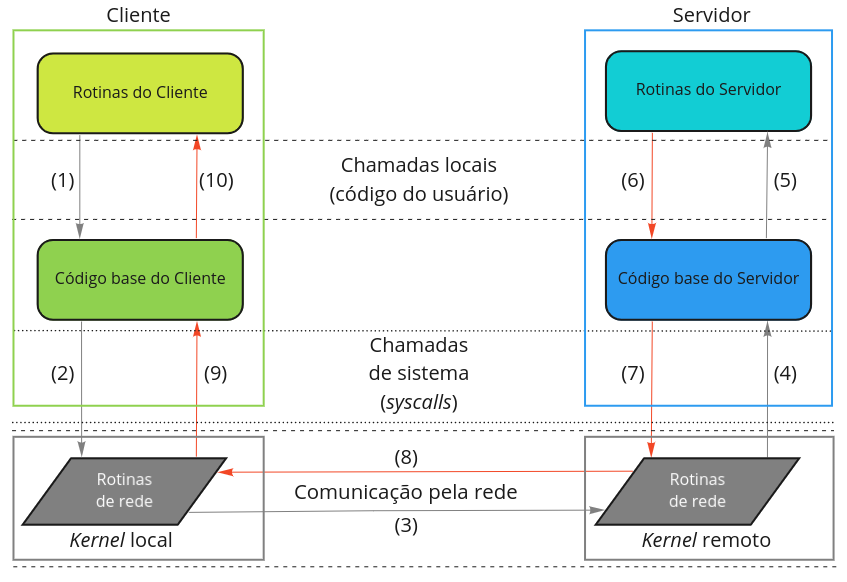
\includegraphics[width=\textwidth]{figuras/diagramas/cap2/cliente_servidor.png} 
    \label{fig:rpc_client_servidor}
\end{figure}

Essa visão simplificada pode ser conferida na Figura \ref{fig:rpc_client_servidor}. Nessa representação, tem-se um cliente, que é o \textit{caller}, e o servidor, que é o \textit{callee}, separados por uma rede física. Existe uma separação lógica para a aplicação, onde o código implementado pelo desenvolvedor é executado apenas nas camadas superiores, compondo as rotinas do cliente e do servidor. Essas rotinas, por sua vez, chamam procedimentos implementados pelo \textit{framework}, representados na Figura \ref{fig:rpc_client_servidor} pelo conjunto dos blocos \textbf{código base do cliente} e \textbf{código base do servidor}. Vale ressaltar que no bloco \textbf{código base do cliente} estão expostas funções que representam as rotinas a serem executados no servidor, de modo a tornar a utilização do RPC transparente para o desenvolvedor, ao reproduzindo o comportamento de funções executadas localmente. O \textbf{código base do servidor} é responsável por registrar os procedimentos remotos escritos pelo desenvolvedor, de modo que o cliente consiga enviar suas requisições para cada um deles de maneira independente. Esse código base também é responsável por interagir com o sistema operacional, de modo a utilizar as funcionalidades do \textit{kernel} para preparar os dados e enviá-los pela rede, cumprindo as etapas da camada de transporte, enlace e física. As setas cinzas representam o percurso dos dados do cliente, enquanto as laranjas representam a resposta do servidor. A ordem de ocorrência de cada etapa da comunicação está numerada na figura para facilitar o entendimento do leitor.

Os \textit{endpoints} num RPC podem ser nomeados de diversas formas: cliente e servidor; nós numa rede \textit{peer-to-peer}; \textit{hosts} de sistema computacional em \textit{grid}; ou até mesmo como microsserviços. Nesse modelo não há restrição para que sejam somente duas entidades, sendo que múltiplos \textit{endpoints} se comunicando são suportados\cite{bergstrom2007anycast}.

Conforme descrito em \cite{birrell1984implementing}, originalmente a ideia de RPC foi desenvolvida com um mecanismo síncrono de requisições e respostas, amarrado a uma linguagem de programação específica e utilizando um protocolo de rede próprio, para que a computação a ser realizada pudesse ser exportada do cliente para o servidor. O objetivo desse sistema era proporcionar a chamada de funções numa máquina remota, com um espaço de endereçamento diferente, a partir das mesmas semânticas encontradas para executar funções localmente. O cliente e o servidor executavam uma única \textit{thread} e funcionavam de maneira síncrona, o cliente enviava uma requisição e ficava bloqueado esperando a resposta do servidor. Tal RPC foi desenvolvido por uma equipe de pesquisa de \textit{internetwork} da empresa Xerox, na década de 1980 e era executado numa LAN pequena e fechada.

\begin{figure}[ht]
    \centering
    \caption{RPC síncrono}
    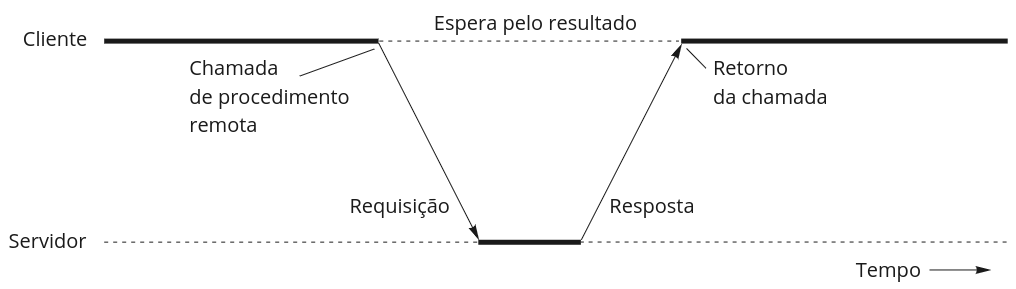
\includegraphics[width=\textwidth]{figuras/diagramas/cap2/rpc_sync.png} 
    \label{fig:rpc_sync}
\end{figure}

\begin{figure}[ht]
    \centering
    \caption{RPC assíncrono}
    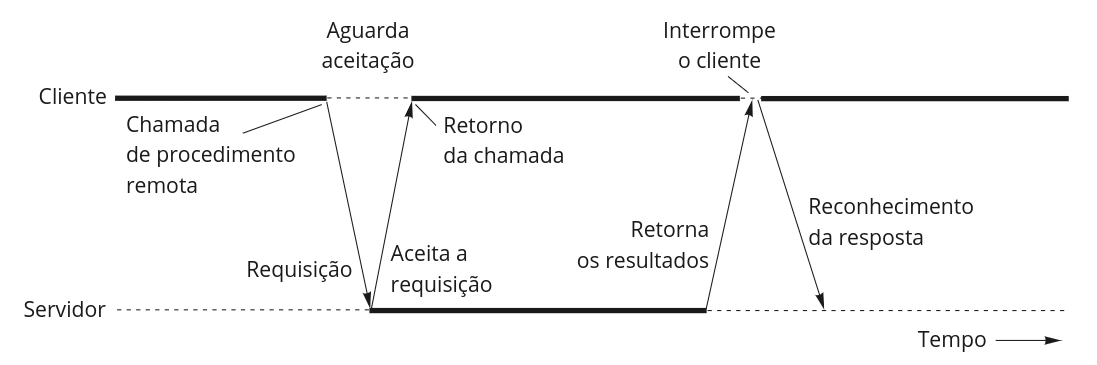
\includegraphics[width=\textwidth]{figuras/diagramas/cap2/rpc_async.png} 
    \label{fig:rpc_async}
\end{figure}

A comparação entre modos síncrono e assíncrono de RPC é melhor observada na Figura \ref{fig:rpc_sync} e na Figura \ref{fig:rpc_async}, respectivamente. Enquanto o cliente fica parado esperando no modo síncrono, no modo assíncrono uma resposta de aceitação da requisição é emitida instantaneamente, e no futuro quando a requisição for de fato processada o servidor enviará a resposta para o cliente. Nesse intervalo o cliente fica livre para executar outras tarefas em paralelo, e ao receber a resposta ele retorna para o fluxo anterior.

Outro aspecto importante dos \textit{frameworks} de RPC modernos foi a introdução de uma camada composta por um compilador e uma IDL (\textit{Interface Definition Language}), contendo arquivos que descrevem textualmente o formato e os tipos dos dados que serão trafegados pela rede, bem como os procedimentos que operam esses dados \cite{slee_thrift_nodate}. Além de servir como uma documentação viva das entradas e saídas do sistema, ainda é possível empregar ferramentas de geração de código, que transformarão os tipos declarados nos arquivos de IDL nos códigos de base do cliente e do servidor automaticamente, de maneira a permitir que o desenvolvimento de aplicações RPC seja mais ágil e simples.

\section{gRPC}

O protocolo gRPC foi criado pelo Google e liberado como um sistema de código aberto em 2015, sendo desenvolvido com o objetivo de permitir a comunicação entre diversos microsserviços utilizados internamente pela empresa. Atualmente serve também como porta de acesso aos diversos serviços externos para os clientes da sua plataforma de computação em nuvem. A comunicação é feita utilizando o protocolo HTTP/2, tendo como serializador e IDL a biblioteca Protobuffers, criada pela mesma empresa.

\subsection{Arquitetura}

O gRPC \cite{google_grpc_2015} é baseado na ideia da definição de serviços, cada um deles contendo um ou mais procedimentos de RPC, com seus parâmetros de entrada e de saída definidos na IDL. Toda essa especificação de tipos de entrada e de saída, serviços e procedimentos de RPC são descritas na sintaxe do Protobuffers em arquivos com a extensão \textbf{.proto}. Após a definição desses arquivos, o desenvolvedor utiliza a CLI (\textit{Command Line Interface}) do compilador do Protobuffers (protoc), que irá gerar os arquivos de base para clientes e servidores nas linguagens que o desenvolvedor escolher, dentre uma vasta gama disponível, tais como C++, C\#, Go, Java, Kotlin, Python, Ruby, etc. Desse modo é possível que clientes e servidores em diferentes linguagens interajam entre si sem dificuldades, conforme mostra a Figura \ref{fig:arquitetura_grpc}.

\begin{figure}[ht]
    \centering
    \caption{Arquitetura do gRPC}
    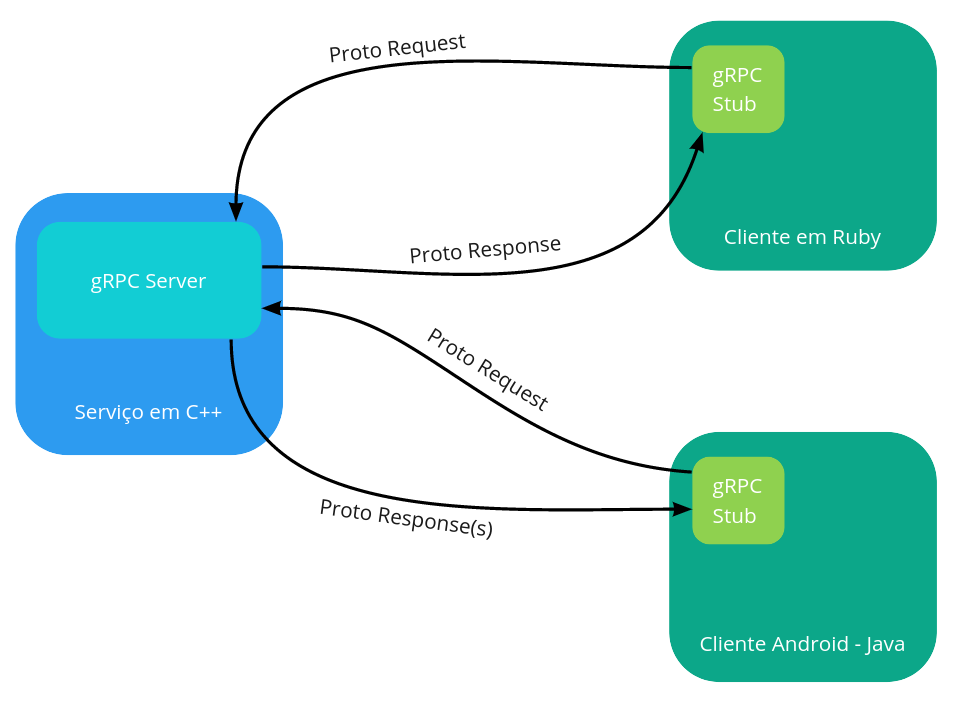
\includegraphics[width=.7\textwidth]{figuras/diagramas/cap2/arquitetura_grpc.png} 
    \label{fig:arquitetura_grpc}
\end{figure}

\subsubsection{Transporte}

Dado o contexto do Google de utilizar o gRPC como porta de entrada para seus serviços de nuvem pela internet, o gRPC é implementado com o protocolo mais comumente utilizado para comunicação na \textit{web}: o HTTP, especificamente sua segunda versão.

O protocolo HTTP/2 introduz algumas melhorias em relação a sua versão anterior, tais como: transportar dados em formato binário ao invés de texto simples, o que proporciona melhores otimizações de codificação e compactação da informação trafegada; multiplexação entre múltiplos \textit{streams} de dados numa mesma conexão, de tal modo que uma única conexão é utilizada para enviar e receber múltiplas requisições do gRPC; e compressão de cabeçalhos para diminuir a quantidade de dados transportados na rede.

O protocolo de camada de transporte utilizado por baixo do HTTP/2 é o TCP, o que permite a oferta de algumas garantias não definidas no HTTP/2. Tais como: a garantia de entrega e ordenação de pacotes, controle de congestionamento e fluxo, entre outras.

\subsubsection{Serialização e geração de código base}

Para transportar os dados, o gRPC faz uso do Protobuffers, também utilizado como linguagem de IDL. Seu compilador é responsável por gerar os arquivos de código que os desenvolvedores utilizam como base para implementar as lógicas de negócio presente nas funções que serão executadas de maneira remota. Tais códigos base são exemplificados na Figura \ref{fig:arquitetura_grpc} e são as caixas nomeadas como \textbf{gRPC Server} e \textbf{gRPC Stub}, que abstraem as lógicas do servidor e dos clientes, respectivamente. Essas abstrações se responsabilizam por permitir que os desenvolvedores se preocupem apenas com a implementação das funções, sem se preocupar com as outras etapas necessárias para a realização do RPC, como por exemplo, lidar com a rede e serialização os dados.

\section{HPRPC}

O HPRPC foi um protocolo RPC concebido com três propósitos em mente: arquitetura simples e leve, alta performance e suporte multiplataforma. O protocolo foi concebido para uso no contexto de HPC, e foi desenhado com arquitetura baseada no gRPC \cite{bagci_lightweight_2016}.

\subsection{Arquitetura}

O protocolo possui uma arquitetura com quatro componentes principais: um controlador, um componente para abstração de chamadas ao protocolo de transporte e outros dois componentes responsáveis por tratar o envio de dados por parte do cliente e recebimento de dados por parte do servidor. 

\begin{figure}[ht]
    \centering
    \caption{Arquitetura do HPRPC}
    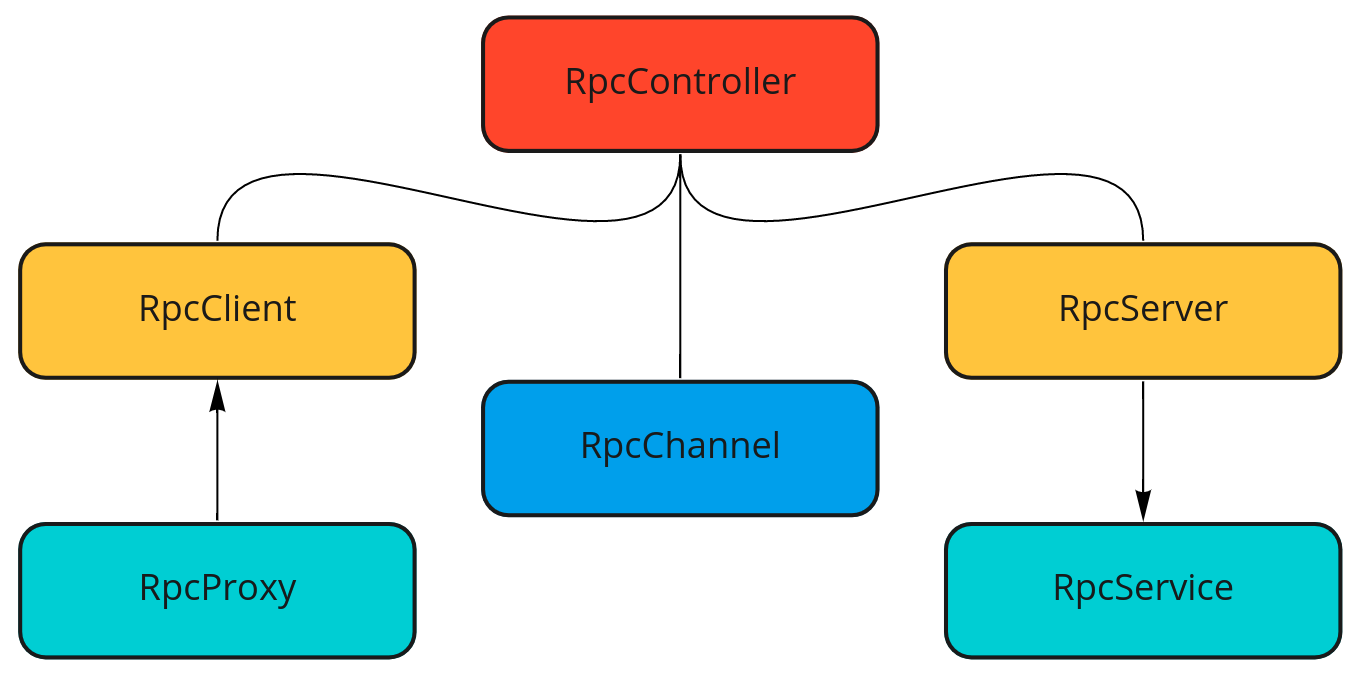
\includegraphics[width=0.7\textwidth]{figuras/diagramas/cap2/arquitetura_hprpc.png} 
    \label{fig:arquitetura_hprpc}
\end{figure}

Na Figura \ref{fig:arquitetura_hprpc} é possível observar o \textbf{RpcController} responsável por enviar mensagens dos clientes para os servidores usando os \textit{channels}. Na mesma imagem também é possível observar o \textbf{RpcChannel} responsável pela camada de comunicação, que implementa os métodos de envio para camada de transporte por TCP. Além desses dois blocos, existem também os blocos \textbf{RpcClient} e \textbf{RpcServer}, que são responsáveis pelo envio de informações do cliente para o servidor através do \textit{channel} e recebimento da resposta correspondente. É interessante notar que no \textbf{RpcClient} existe o \textbf{RpcProxy}, 0 \textit{proxy} consiste em classes geradas que fazem a abstração do transporte para que a chamada do RPC seja transparente ao programador. O último dos blocos é o \textbf{RpcService}, que consiste em uma classe customizada gerada que sobrescreve métodos do bloco \textbf{RpcServer}, para fornecer uma maneira de invocar o método correto do serviço.

\subsection{Cabeçalhos}

O cabeçalho do HPRPC possui quatro atributos. O primeiro atributo é o \textbf{id}, que armazena o identificador da mensagem, esse campo é importante para associar uma resposta a uma requisição. Outro campo disponível no cabeçalho é o \textbf{MsgType}, que indica se a mensagem em questão é uma chamada de RPC, uma resposta, uma resposta vazia, um erro, uma notificação de canal fechado ou uma mensagem sem tipo. Além desses, existem outros dois campos \textbf{ProcType} e \textbf{SrvType}, que indicam quais os serviços e procedimentos remotos a serem executados. O diagrama da classe \textbf{RpcHeader} pode ser visto na Figura \ref{fig:cabecalho_hprpc}.

\begin{figure}[ht]
    \centering
    \caption{Cabeçalho do HPRPC}
    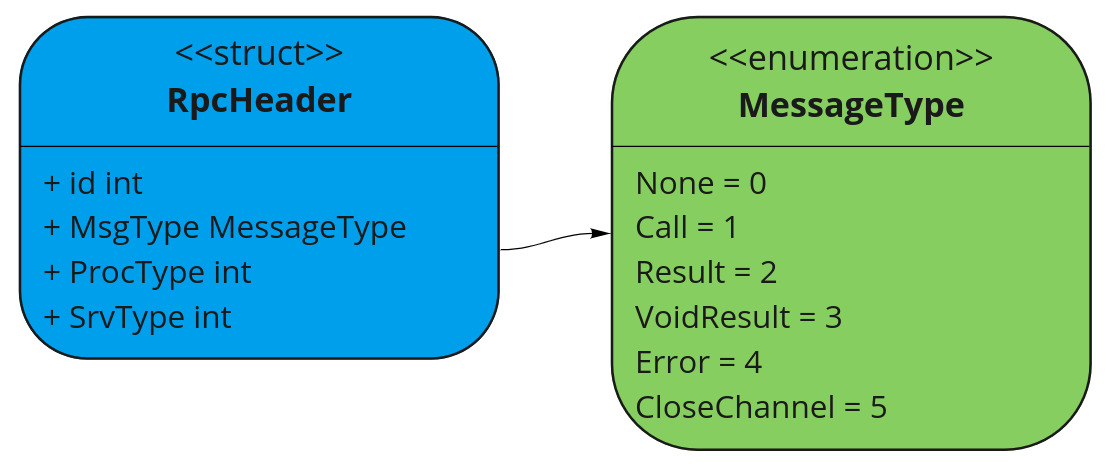
\includegraphics[width=0.6\textwidth]{figuras/diagramas/cap2/cabecalho_hprpc.png} 
    \label{fig:cabecalho_hprpc}
\end{figure}

\subsection{Limitações}

O HPRPC foi desenvolvido com simplicidade como um dos pilares, por essa razão algumas limitações foram impostas ao protocolo e estão listadas abaixo:

\begin{itemize}
	\item Chamadas síncronas - O HPRPC não suporta nativamente execução de procedimentos remotos de forma assíncrona.
	\item Cliente e servidor únicos - Somente um nó cliente e um nó servidor são suportados pelo protocolo.
	\item Plataformas homogêneas - O HPRPC foi implementado em diversas linguagens, entretanto, aplicações se comunicando a partir de linguagens distintas não podem ter \textit{endianness} (ordenação de bytes) divergentes, além disso, outra limitação é que a codificação de \emph{strings} deve ser idêntica, em essência os dados das linguagens não podem divergir de forma a gerar inconsistência entre o que é enviado e recebido.
\end{itemize}

\subsection{Serialização de dados}

Os autores do HPRPC implementaram um serializador próprio, chamado de KodoSis. Ele é a principal melhoria do HPRPC sobre o gRPC no contexto de HPC, possuindo um mecanismo de serialização simplificado que dispensa a necessidade de identificadores por campo.

A estratégia de suprimir identificadores nos campos serializados incorre na geração de uma sequência de dados serializados de tamanho menor, que implica em uma quantidade menor de dados transmitidos e por fim em um tempo menor de execução, quando comparado ao gRPC.

É importante ressaltar que o ganho de desempenho associado às simplificações do HPRPC restringem a implementação de diversos mecanismos, que o gRPC possui, para facilitar desenvolvimento e manutenção das aplicações RPC. Entre essas, é possível citar o suporte a argumentos opcionais e o versionamento de protocolo.

O KodoSis usa uma IDL própria a fim de normalizar o formato de dados e automatizar a geração de código para as linguagens suportadas. Atualmente o HPRPC e o KodoSis suportam C\# com .NET e C++.

Deve-se notar que o KodoSis foi otimizado para serializar listas de tipos básicos de modo a gerar o menor dado serializado possível, dessa forma, os testes propostos pelo artigo estudado foram construídos com foco em listas de \textbf{int32} e \textbf{double}, para os quais o tempo de execução e o desempenho são melhores que o gRPC.

\section{Thrift}

O Thrift \cite{slee_thrift_nodate} foi desenvolvido no Facebook como um ambiente escalável para desenvolvimento de serviços entre diversas linguagens de programação. Seu objetivo principal é permitir que serviços heterogêneos possam se comunicar de maneira eficiente e confiável.

Isso é solucionado através de uma linguagem neutra, uma IDL, na qual desenvolvedores podem definir interfaces de serviços e seus respectivos tipos de dados, de modo que todo código necessário para estabelecer chamadas remotas de procedimentos entre clientes e servidores possa ser gerado automaticamente a partir dessas definições.

\subsection{Tipos}
A especificação define sete tipos básicos de dados: booleano; byte acompanhados de sinal; inteiros de 16, 32 e 64 bits acompanhados de sinal  (\textbf{int16}, \textbf{int32}, \textbf{int64}); número de ponto flutuante com resolução de 64 bits (\textbf{float64}); textos agnósticos de codificação, que podem representar sequências binárias ou de caracteres (\textbf{binary} ou \textbf{string}).

Também são definidos quatro tipos complexos de dados: estruturas de dados, como um tipo comum representativo de um objeto, também chamado de \textit{struct}; \textit{containers}, especificamente listas, conjuntos e mapas de dados; exceções, como estruturas de dados especificas para tratamento de erro; e serviços, que servem como um definições para os procedimentos que podem ser executados remotamente entre clientes e servidores.

\subsection{Transporte}
O Thrift normalmente é utilizado sobre os protocolos TCP/IP, mas isso não é um requisito. Sendo possível definir qualquer tipo de transporte a ser usado. A especificação define um conjunto básico de métodos necessários para que o sistema possa ler e escrever dados por qualquer meio de comunicação a ser implementado.

\subsection{Protocolo}
Este \textit{framework} define uma estrutura básica de mensagens que encapsulam os dados trocados entre cliente e servidor. Entretanto, ele não especifica um único formato para serialização de dados. Em contrapartida, sua especificação define um conjunto genérico de métodos a serem disponibilizados por qualquer tipo de codificador em um formato específico implementado para interagir com o Thrift. Os métodos definidos focam na escrita e leitura dos diferentes tipos de dados, assim como na definição da estrutura básica das mensagens.

\subsection{Compilador e IDL}
O compilador do Thrift é implementado em C++ e utiliza os programas \emph{lex} e \emph{yacc} para fazer a análise léxica e processar o código de sua IDL. A geração do código utilizado para estabelecer a comunicação RPC é feita em duas etapas. Inicialmente é executada a resolução de arquivos externos importados pela IDL, depois as definições de tipos são resolvidas e analisadas por verificadores de erros. Por fim, é gerado o código a partir da árvore sintática da IDL, que cria as interfaces a serem implementadas pelos métodos definidos, assim como a lógica necessária para interagir com meio de transporte escolhido, instanciar os servidores e clientes para comunicação e codificar os dados no formato implementado.

É possível analisar um exemplo de uma IDL do Thrift no Código \ref{alg:example.thrift}.

\includecode[Thrift]{Código exemplificando o uso da IDL do Thrift} {alg:example.thrift}{codigos/example.thrift}{Adaptado da documentação do Thrift (\url{https://github.com/apache/thrift/blob/master/tutorial/tutorial.thrift})}

O estudo dos \textit{frameworks} de RPC apresentados neste capítulo, juntamente com o referencial teórico, demonstram a diversidade e robustez dos \textit{frameworks} de RPC utilizados nos dias atuais. Neste sentido, no capítulo a seguir são apresentadas as decisões arquiteturais tomadas para o aRPC, bem como as justificativas para as mesmas. São também apresentados paralelos com soluções alternativas e cada um dos componentes do aRPC são minunciosamente detalhados.
